\documentclass[letterpaper,11pt]{article}

\usepackage[margin=1.0in]{geometry}
\usepackage{amsmath}
\usepackage{amsthm}
\usepackage{amsfonts}
\usepackage{algorithm2e}
\usepackage{url}
\usepackage{fancyhdr}
\usepackage{blkarray}
\usepackage{graphicx}
\usepackage{csquotes}
\usepackage{cite}
\pagestyle{fancy}
\lhead{Algorithmic-Trading Summary --- Fall 2018}
\rhead{}


\begin{document}
\thispagestyle{plain}
\noindent{Algorithmic-Trading --- Fall 2018}

\noindent{Alex Thomas}

\noindent{Colgate University} \\

\noindent\textbf{Relative Strength Index (RSI)}

\section*{Introduction }

Relative Strength Index (RSI) is a momentum indicator that measures the magnitudes of price changes to analyze overbought or oversold stocks. It demonstrates a particular security's recent performance over a relatively short window compared to the mean. This indicator is widely used today in algorithmic trading. 

\section*{Motivations and Measures}
RSI is an indicator that takes advantage of momentum and is a value between 0 and 100. The equation for RSI is $RSI = 100.0 - (100.0 / (1.0 + RS))$ \cite{Chong2014}. RS is defined as average gain of up periods divided by the average gain of down periods over a specified window. Therefore, a large RSI value is indicative of stocks that have had recent larger gains compared to losses while a low RSI value is indicative of stocks with poor recent performance compared to the mean.

\section*{Key Techniques}
Our implementation uses a very simple method. Sell signals are generated when the RSI is over 70 and buy signals are generated when the RSI is under 30. This is very logical, as expected gains are the largest when a stock has performed poorly recently and is expected to revert back to the mean. This strategy also uses a 14 day window, which is standard across the industry. 

\begin{figure}[ht!]
\centering
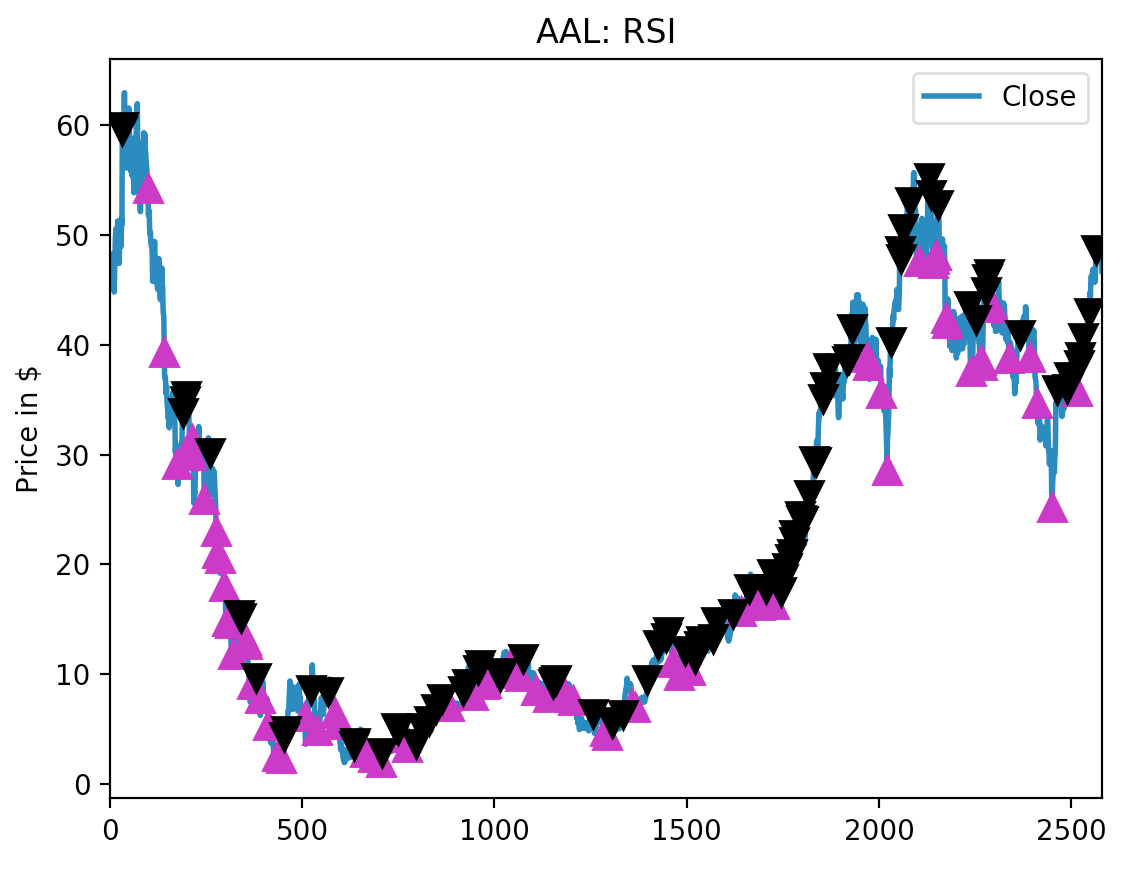
\includegraphics[width=90mm]{AAL_RSI_signals.png}
\caption{RSI Strategy applied to AAL\label{overflow}}
\end{figure}

\begin{figure}[ht!]
\centering
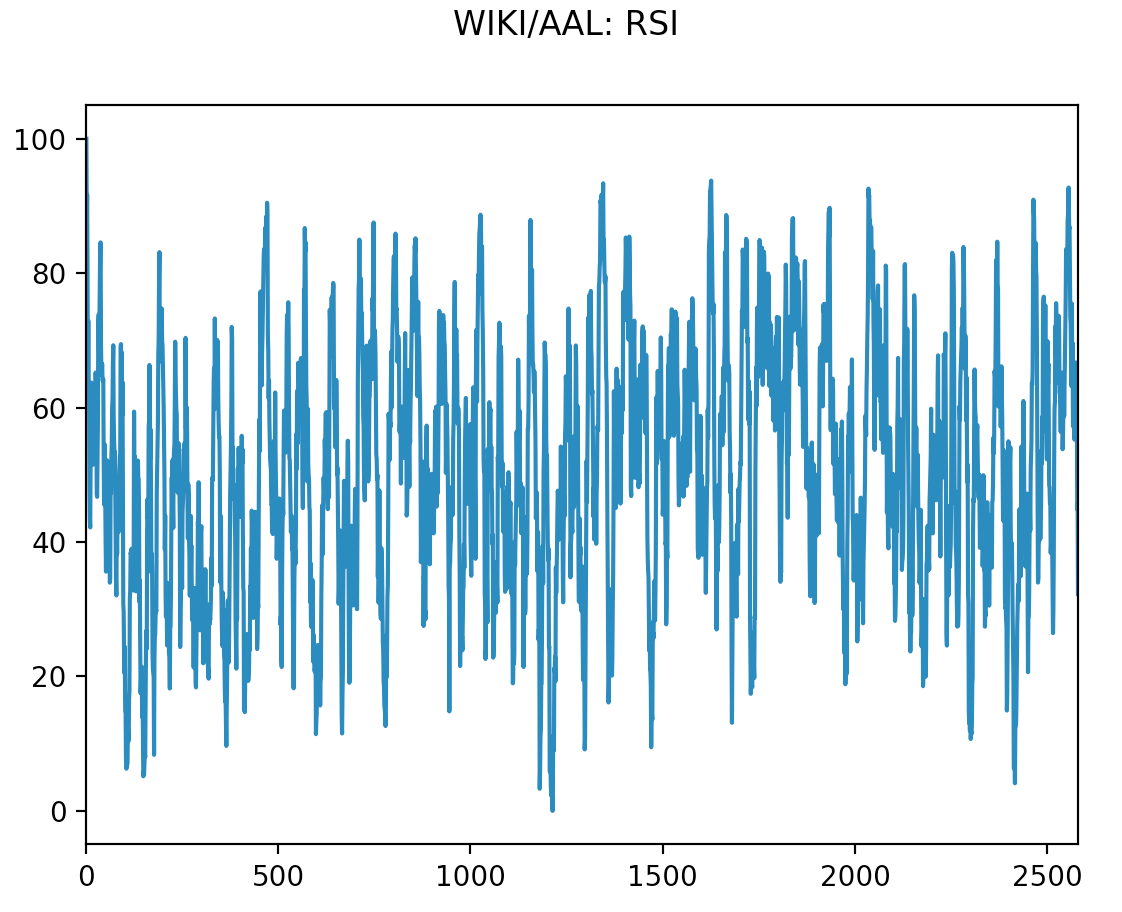
\includegraphics[width=90mm]{AAL_RSI.png}
\caption{ RSI of AAL \label{overflow}}
\end{figure}

\section*{Analysis}

\subsection*{Effectiveness}
This strategy takes advantage of over-purchasing or overselling of securities to predict convergence back to the mean. So, like Bollinger Bands this strategy does take advantage of mean reversion. Our implementation uses simple moving average as a basis. However, numerous papers have cited that RSI isn't very effective in stock market forecasting \cite{Chong2014}.

\subsection*{Runtime}
The components to consider for this strategy include pulling stock data into a Pandas data frame and calculating rolling means from the data-frame and marking their differences. Pandas is a python data analysis package and is perhaps the most powerful open source data analysis or manipulation tool available. For each calculation, it has to scrape through the entire data-frame at a rolling window, giving a linear runtime.

\subsection*{Quality Metric}
The strategy is tested against a baseline long position of 100 shares of a given stock. Therefore, we compare the strategy against simply buying 100 shares of stock right at the opening date and then sell at the final date. For our implementation, over 15 different stocks were chosen and run against this baseline. Unfortunately, most RSI implementations didn't outperform the baseline. The performance was comparable to EMA but slightly worse, as we do see more stocks not beating out the baseline. GOOG beat the baseline by 12.88\% while on the other hand DIS massively underperformed and posted a -7.08\% performance. It would be interesting to see how RSI performs on intra-day data.

\subsection*{Space / Memory Implications}
The only space for  RSI required is the data-frame, which is very reasonable.

\section*{Conclusion}
RSI doesn't prove to be a terribly effective strategy. However, we do notice better performance than some of the other simple momentum strategies. With all of these relatively simple momentum strategies, it is very apparent that each on its own isn't entirely profitable. Next, we will investigate how combining multiple of these measures into one strategy will perform.

\section*{Implementation}
\begin{verbatim}
def execute(stock1, stock2, start_date, end_date):
    stock = stockDataRetriever(stock1, start_date, end_date).getStock()

    # set Pandas df with both stocks
    df = pd.DataFrame(index=stock.index)

    # create measures of up and down performance
    delta = stock['Close'].diff()
    roll_up = delta[delta > 0].rolling.mean()
    roll_down = delta[delta > 0].rolling.mean()
    
    # create RSI
    RS = roll_up/roll_down
    RSI = 100.0 - (100.0 / (1.0 + RS))

    # create the buy and sell commands
    df['buy'] = np.where(RSI < 30, 1, 0)
    df['sell'] = np.where(RSI > 70, -1, 0)
    df['signal'] = df['buy'] + df['sell']

    # when signal changes from 1 to 0 or 0 to 1 - is a buy or sell
    df[positions] = df[signal].diff()

\end{verbatim}

\bibliographystyle{plain}
\bibliography{References}

\end{document}